\section{Encoding Attribute Sequences}
\label{sec:ordering}


\begin{figure*}[t!]
%\begin{minipage}{2\linewidth}
%\begin{subfigure}[c]{0.96\linewidth}
%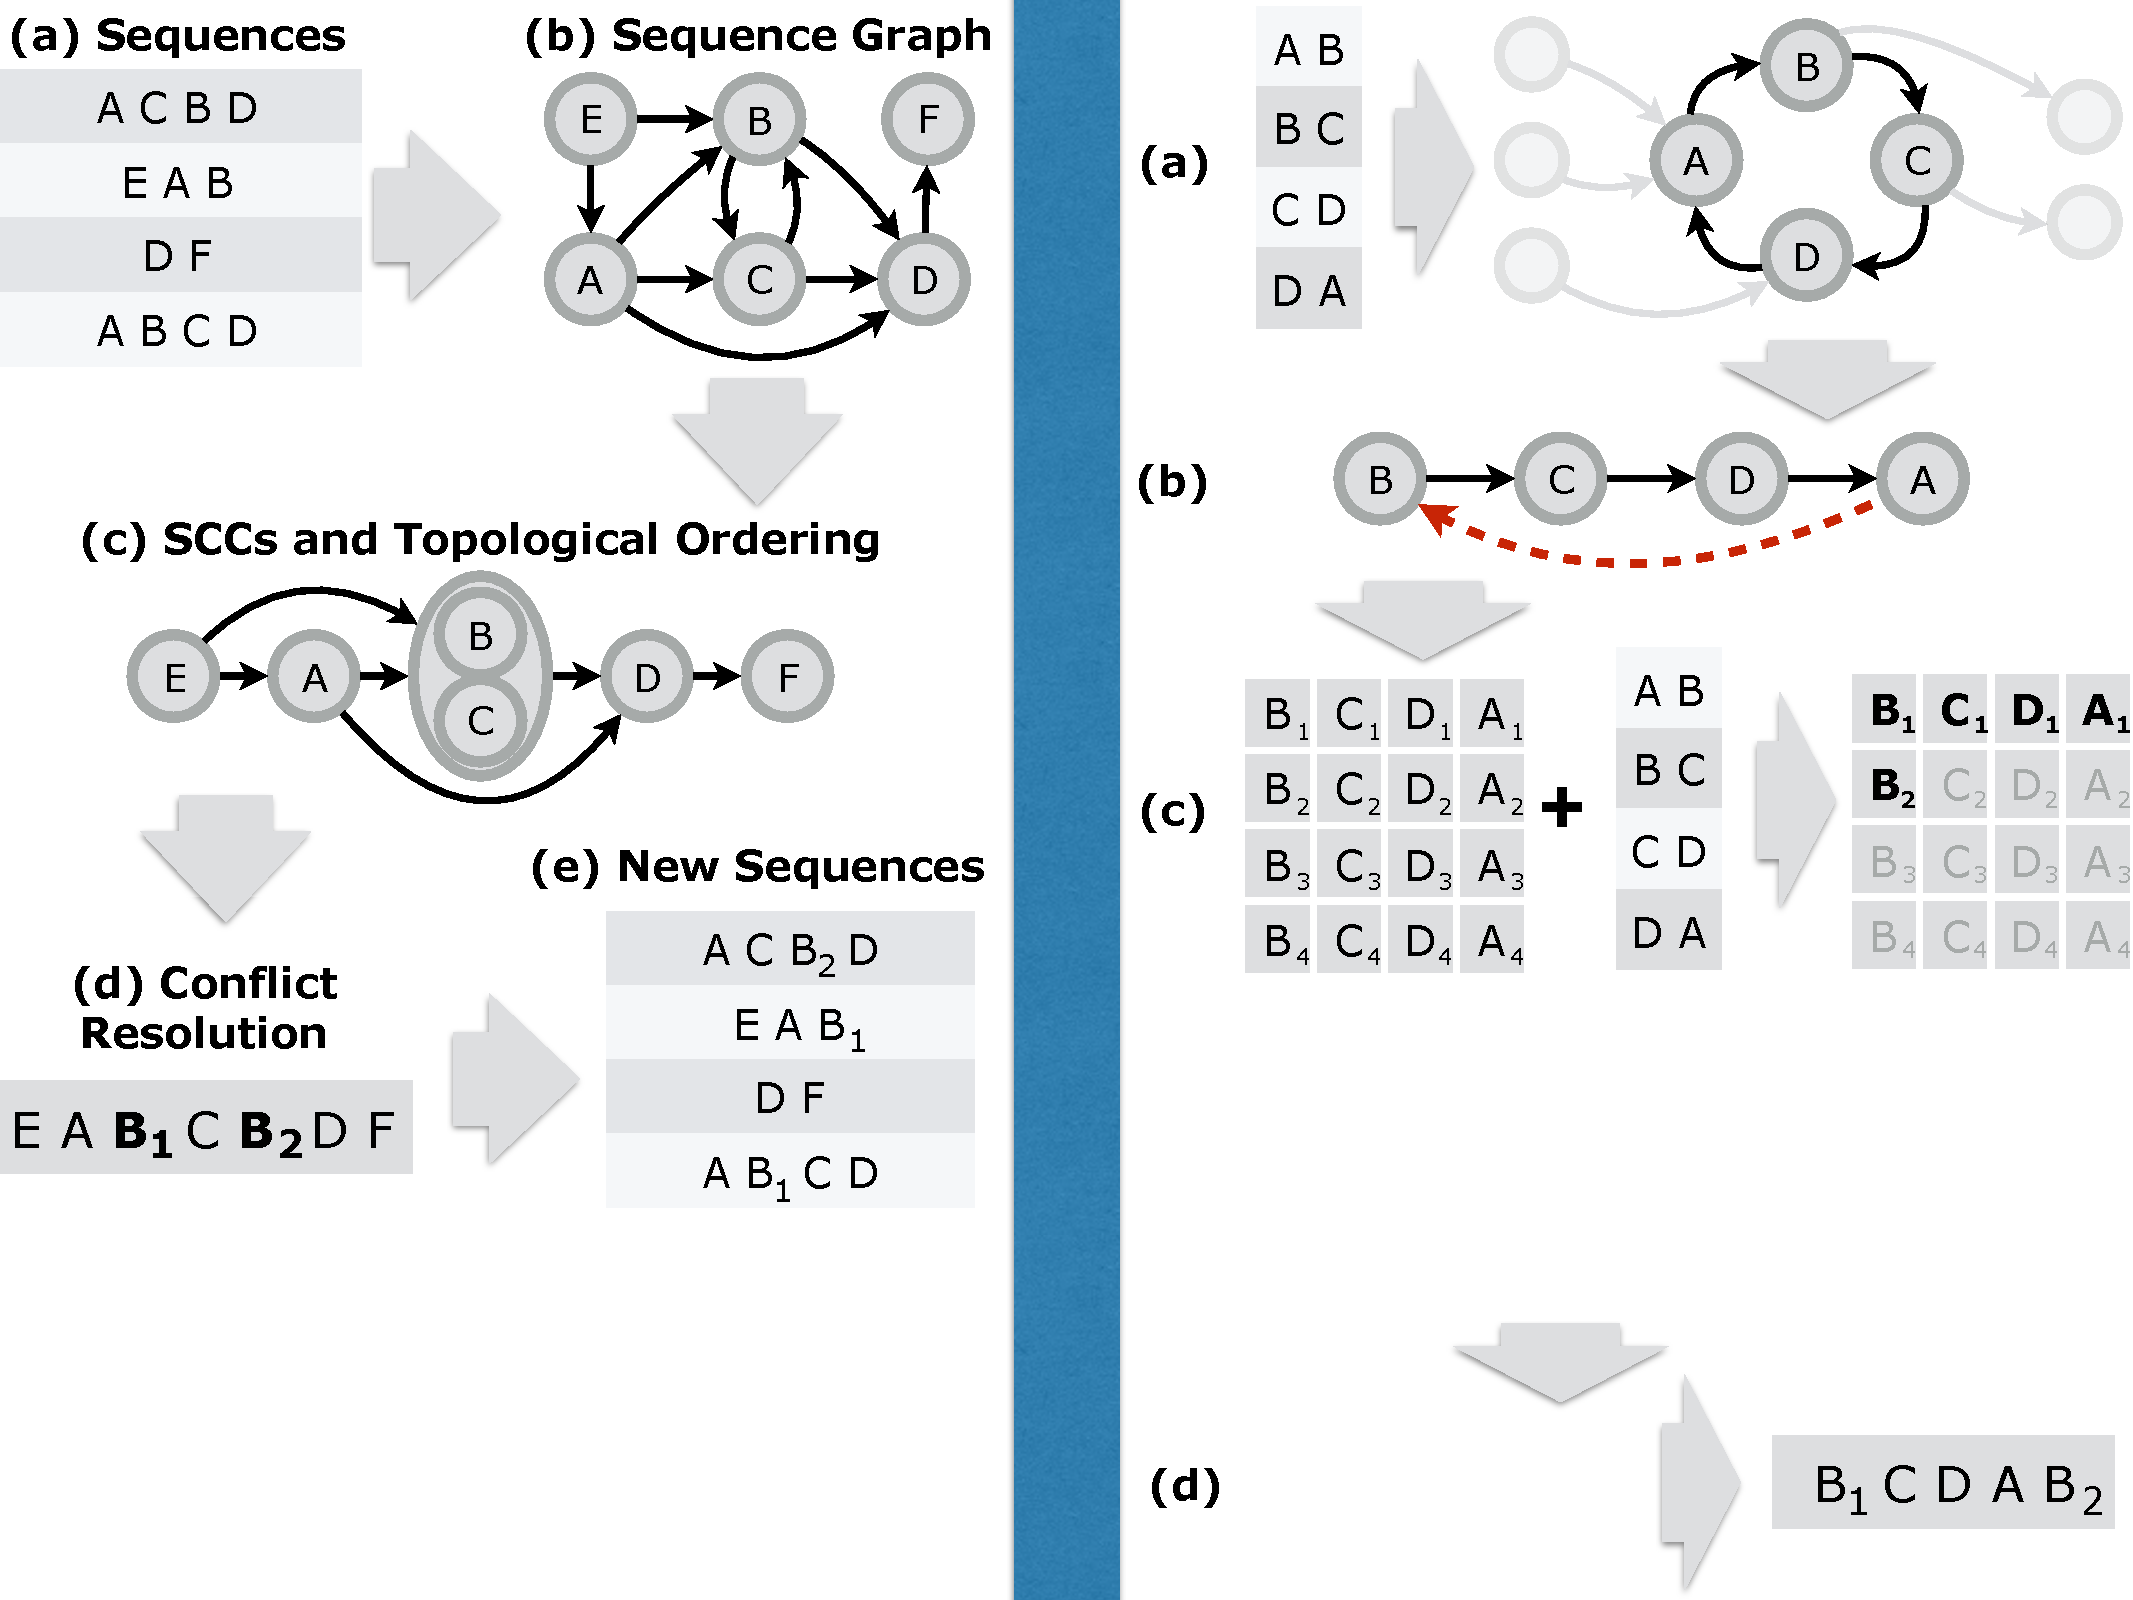
\includegraphics[trim={0 6cm 19.2cm 0}, clip, width=\linewidth]{figures/partial_ordering}
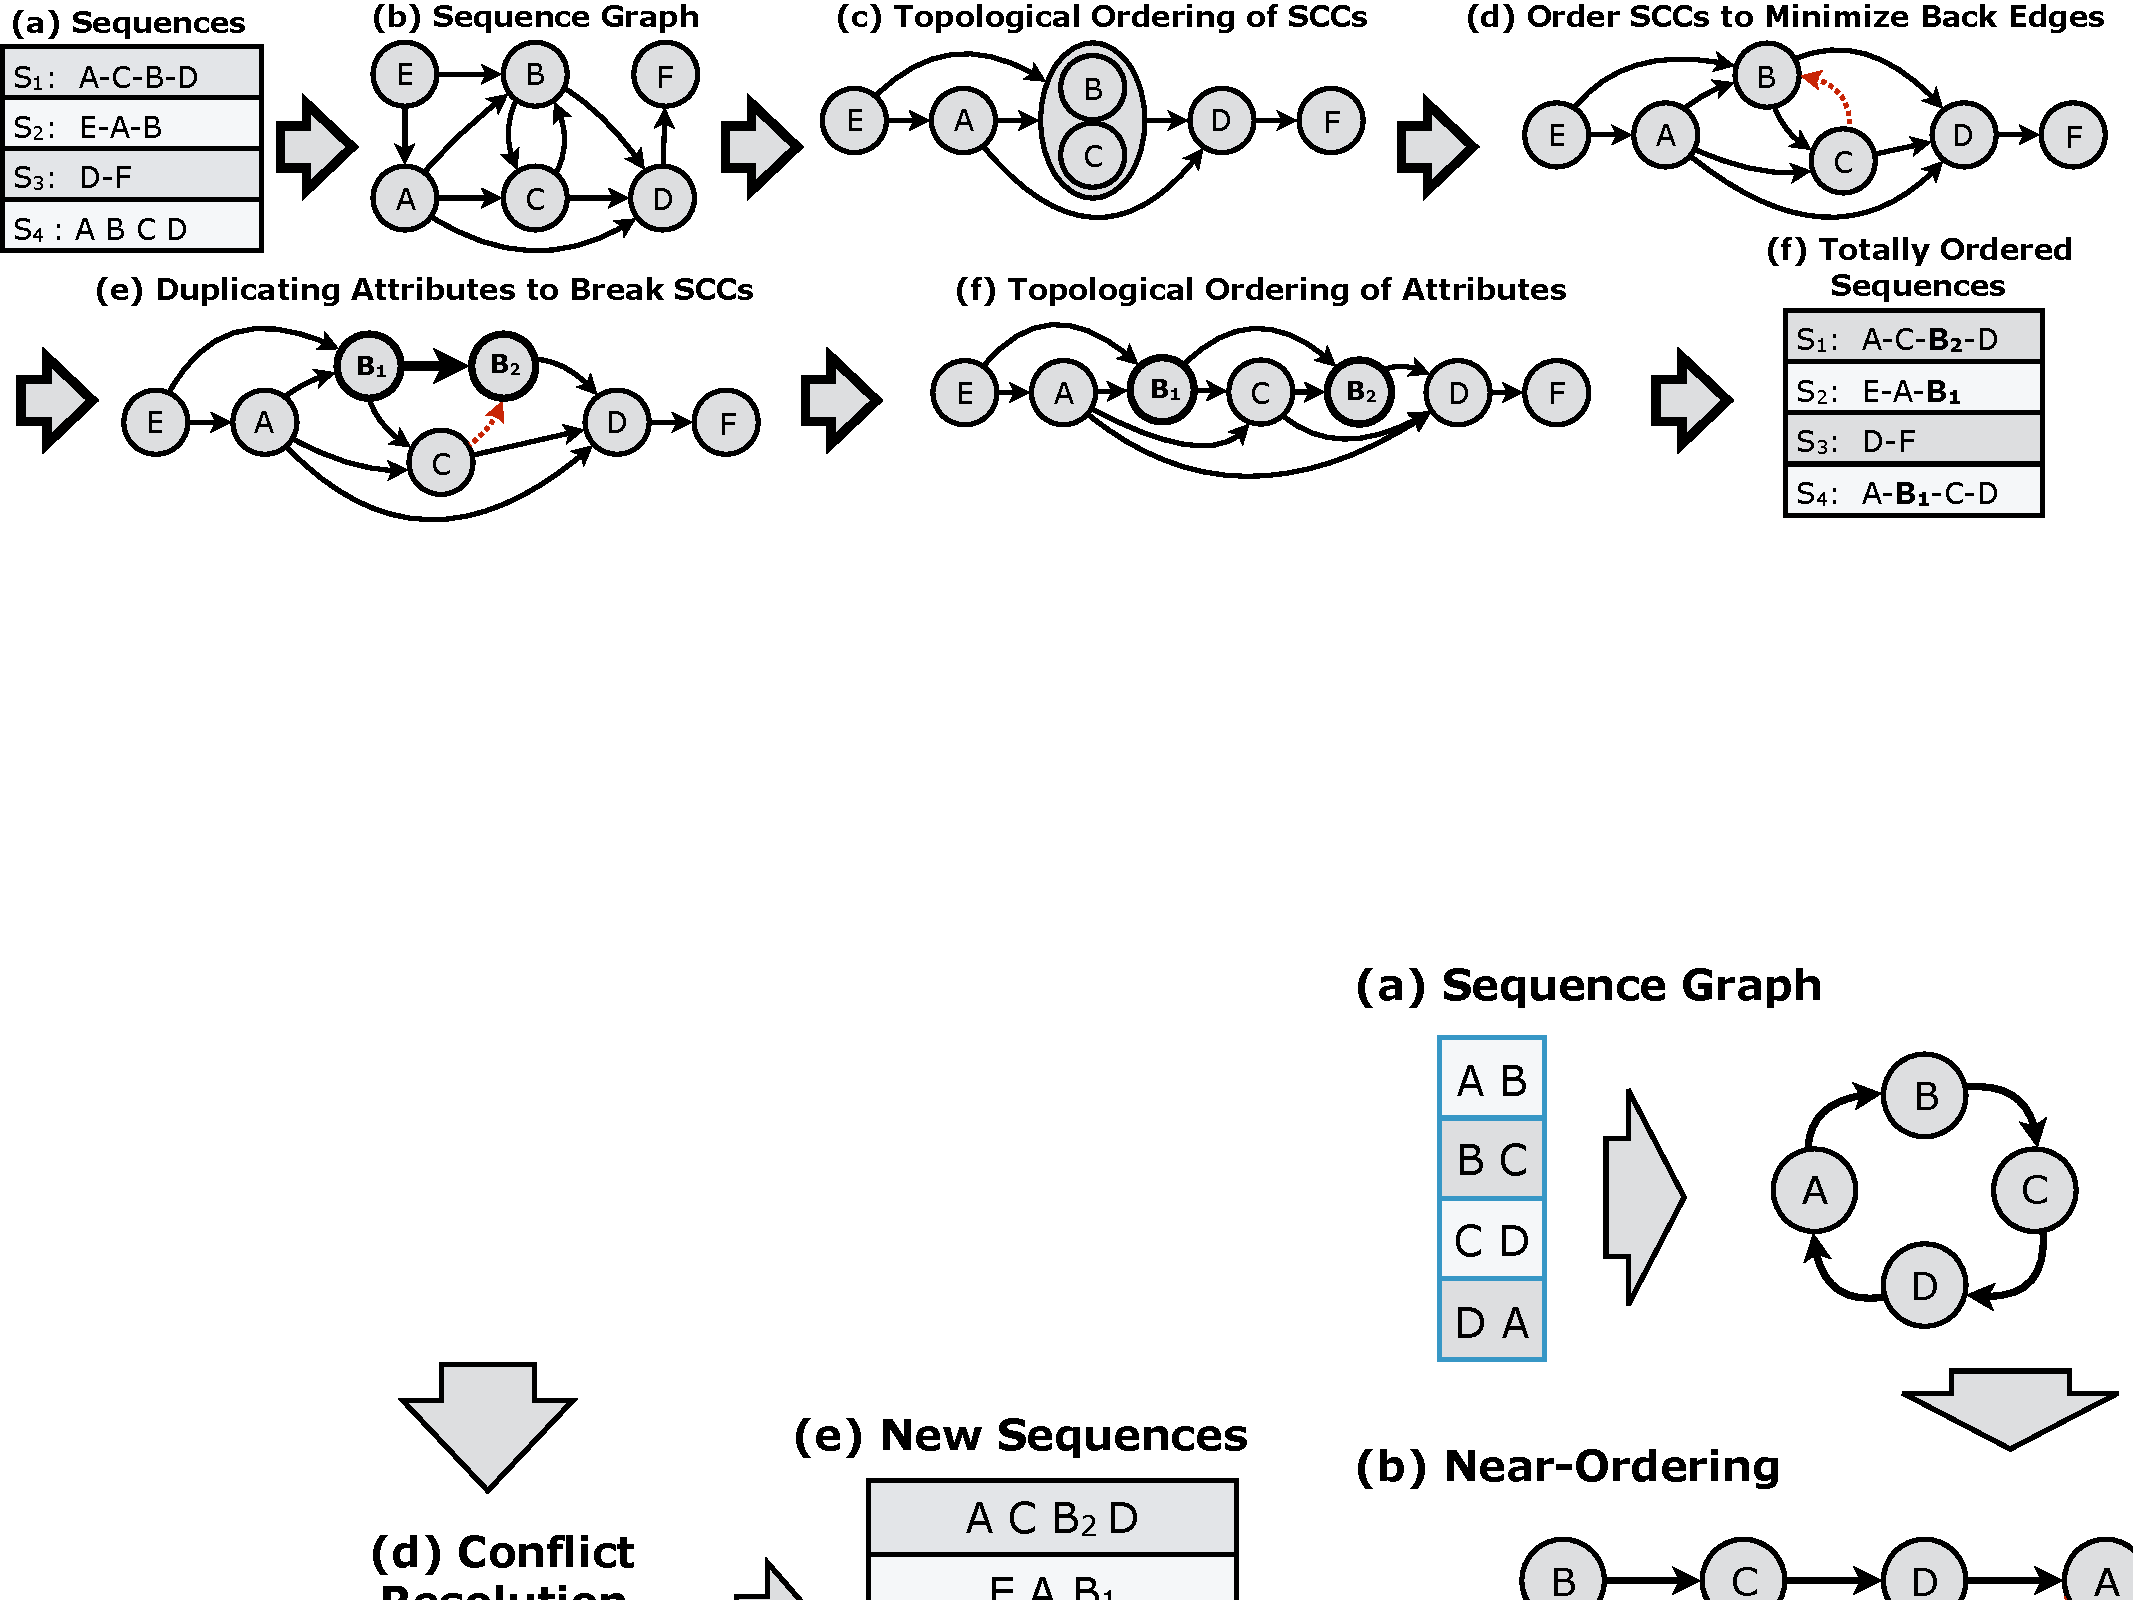
\includegraphics[trim={0 18cm 0 0}, clip, width=\textwidth]{figures/partial_ordering2}
%\end{subfigure} 
%\end{minipage} 
\caption{Sequences forming a cycle of attributes. (a) shows the four input sequences. (b) illustrates the corresponding sequence graph $G$ (c) shows the disjoint SCCs (Strongly Connected Components) of $G$. Each SCC corresponds to a set of incomparable elements. In (d), we order the elements of the SCC to minimize backward edges. (e) and (f) show how nodes of the SCC can be split to make all backward edges become forward edges, allowing a complete ordering to be found. Splitting nodes results in duplicated elements, which slightly changes the original sequences, as shown in (f).}
\label{fig:ordering}
\end{figure*}

In some applications, the \emph{order} of attributes is important.  For example, in service chaining, traffic must traverse middleboxes in a specified order.  In this section, we extend our scheme for encoding \emph{sets} of attributes to support \textit{sequences} of attributes.  We first propose a simple representation of the attribute sequences in a sequence graph.  Next, we discuss how to encode sequences when the attributes follow a partial order.  Then, we show how to encode sequences in general, even when the attributes do not form a partial order.

\subsection{Sequence Graph of Attribute Orderings}
When the tag must encode a sequence of attributes, we need an effective way to identify what \emph{ordering} of attributes can occur.  Figure~\ref{fig:ordering}(a) shows four equivalence classes ($S_1$-$S_4$) with different sequences of attributes ($A$-$F$); for example, $S_2$ has the attribute sequence $E$-$A$-$B$, whereas $S_4$ has $A$-$B$-$C$-$D$.  We can generate a \emph{sequence graph} where each node is an attribute, and a directed edge from node $u$ to node $v$ exists if $u$ appears before $v$ in any of the sequences.  For example, the sequence graph in Figure~\ref{fig:ordering}(b) has an edge from $E$ to $A$, 
from $E$ to $B$, and from $A$ to $B$ because of $S_2$, and from $D$ to $F$ because of $S_3$.  Each sequence in the input data corresponds to a path through the sequence graph.  If the sequence graph is acyclic, the attributes form a partial order, making it easier to encode all of the sequences concisely.

We expect that many use cases impose a natural order on the attributes.  For example, in traffic steering, typically a compression middlebox would typically occur before an encryption middlebox, and encryption would occur before decryption.  Similarly, a firewall would usually appear before a network address translator, so the firewall can act on the end-host IP addresses rather than the address of the NAT.  Still, sometimes exceptions can easily arise.  In designing our techniques for encoding sequences, we optimize for the case where attributes ``mostly'' follow a natural order, and handle the (presumably) small number of exceptions as they arise.

\subsection{Sequences Forming a Partial Order}
If all of the attributes form a (partial) order, we can easily construct a single ordered list of all attributes where each input sequence is a subsequence. We refer to such a sequence as a \emph{supersequence}.  A supersequence can be computed by processing the nodes of the (acyclic) sequence graph in order. For example, suppose the input sequences are $X$-$Y$, $Y$-$Z$, and $X$-$Z$; then, the resulting supersequence would be $X$-$Y$-$Z$. To generate the tags, Algorithm~\ref{alg:memory_min} can be used ``as is'' to generate a concise encoding.  The resulting rules in the switches would simply match on the attributes in the appropriate ``order'', \eg, a rule that checks for attribute $Y$ would include a $0$ bit for $X$, to ensure that middlebox $X$ was already visited (if necessary) and the associated bit in the tag cleared.  We discuss how to compute the rules in more detail in \S~\ref{s:order-rules}.

\subsection{Sequences Forming a Cycle}
\label{ss:breakcycle}
When the sequence graph contains a cycle, no supersequence of attributes exists that is consistent with all of the input sequences.  For example, the sequence graph in Figure~\ref{fig:ordering}(b) contains a cycle with attributes $B$ and $C$ because $S_1$ has sequence $A$-$C$-$B$-$D$ (with $C$ before $B$) while $S_4$ has sequence $A$-$B$-$C$-$D$ (with $B$ before $C$).

\textbf{Group sequences with consistent attribute orderings (Approach I):} The approach merges groups only if they have consistent ordering of the attributes.  For example, $S_2$ and $S_4$ could merge because $E$-$A$-$B$-$C$-$D$ is consistent with both sequences.  Pairs of groups could merge based on similar
criteria as in \S~\ref{ssec:merge}, subject to the constraint on consistent attribute order.  At the completion
of the algorithm, each group would be assigned a group id and a single ordering of their combined attributes, represented as a bitmask.

\textbf{Break cycles by duplicating nodes in the sequence graph (Approach II):} The first approach can sometime result in too many groups that cannot merge. The second approach is more flexible by allowing the merging of two sequences even if they impose a different order on some attributes.  To resolve the inconsistency, we break cycles by \emph{duplicating} some nodes in the sequence graph, and representing each ``copy'' of the attribute with a different bit in the bitmask.  For example, we can break the cycle in Figure~\ref{fig:ordering}(b) by splitting node $B$ into $B_1$ and $B_2$.  This makes it possible to construct a supersequence $E$-$A$-$B_1$-$C$-$B_2$-$D$-$F$ (Figure~\ref{fig:ordering}(f)) that is consistent with each sequence (Figure~\ref{fig:ordering}(g)).

To break cycles in a systematic fashion, we run an algorithm that finds the Strongly Connected Components (SCCs) on the sequence graph.  An SCC is a set of nodes such that for every pair of nodes $u$ and $v$ in the set, $u$ has a directed path to $v$ and vice versa. In this context, every SCC corresponds to a set of attributes that cannot be placed in order.  Figure~\ref{fig:ordering}(c) shows the result of finding SCCs on the sequence graph, identifying the pair of attributes $B$ and $C$. We then identify a minimal set of ``back edges'' to remove, and split nodes to remove each of these back edges.  For example, creating nodes $B_1$ (with an edge \emph{to} $C$) and $B_2$ (with an edge \emph{from} $C$) breaks the cycle, resulting in the acyclic sequence graph in Figure~\ref{fig:ordering}(e) which is redrawn in Figure~\ref{fig:ordering}(f) to highlight a suitable ordering of the attributes, leading to the modified input sequences in Figure~\ref{fig:ordering}(f).  Now, we can simply run Algorithm~\ref{alg:memory_min} ``as is'' to generate the groups and their corresponding bitmasks.

%
%\begin{figure}[t!] 
%\begin{minipage}{1\linewidth}
%\begin{subfigure}[c]{0.96\linewidth}
%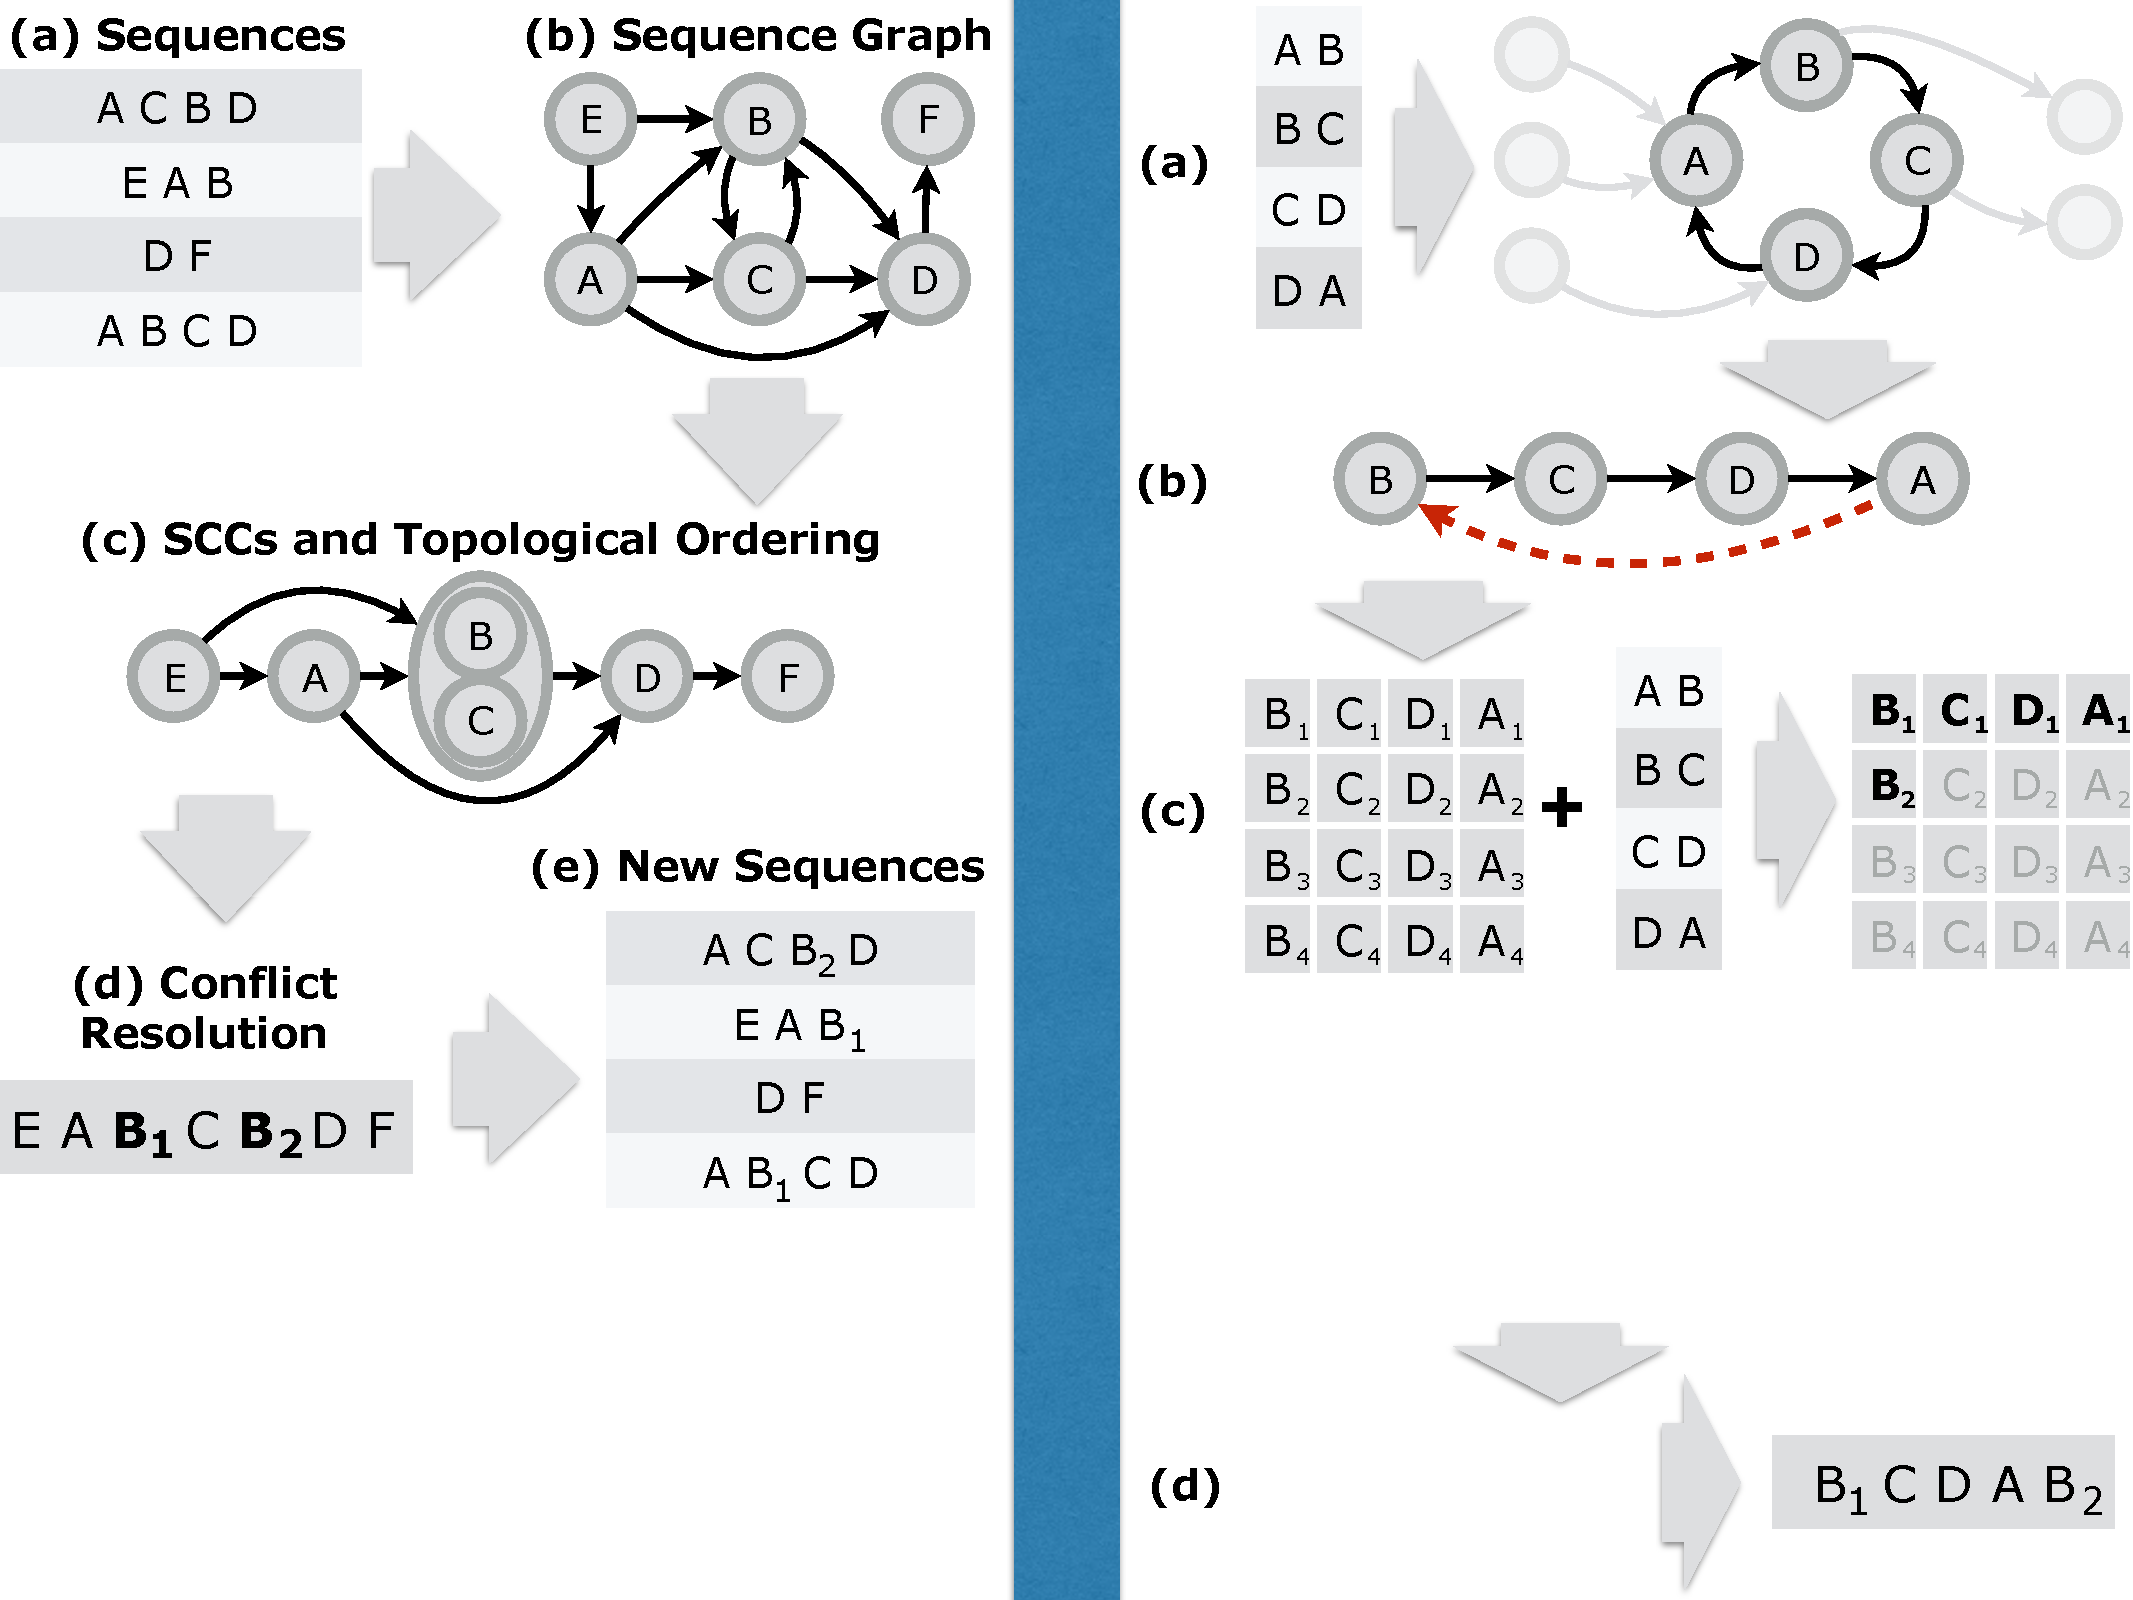
\includegraphics[trim={0 6cm 19.2cm 0}, clip, width=\linewidth]{figures/partial_ordering}
%\end{subfigure} 
%\end{minipage} 
%\caption{Not-aligned ordering constraints. (a) shows the four input ordered sequences. In (b) illustrates the corresponding sequence graph $G$.. (b) shows the disjoints SCCs  (Strongly Connected Components) of $G$. Each SCC corresponds to a set of incomparable elements. (d) describes the result of splitting elements to resolve order-inconsistency, which is covered in more depth in figure \ref{fig:conflict_res}. In (e), the original sequences are modified with the splits such that each sequence adheres to the constructed ordering.}
%\label{fig:ordering}
%\end{figure}



%\begin{figure}[t!] 
%\begin{minipage}{1\linewidth}
%\begin{subfigure}[c]{0.96\linewidth}
%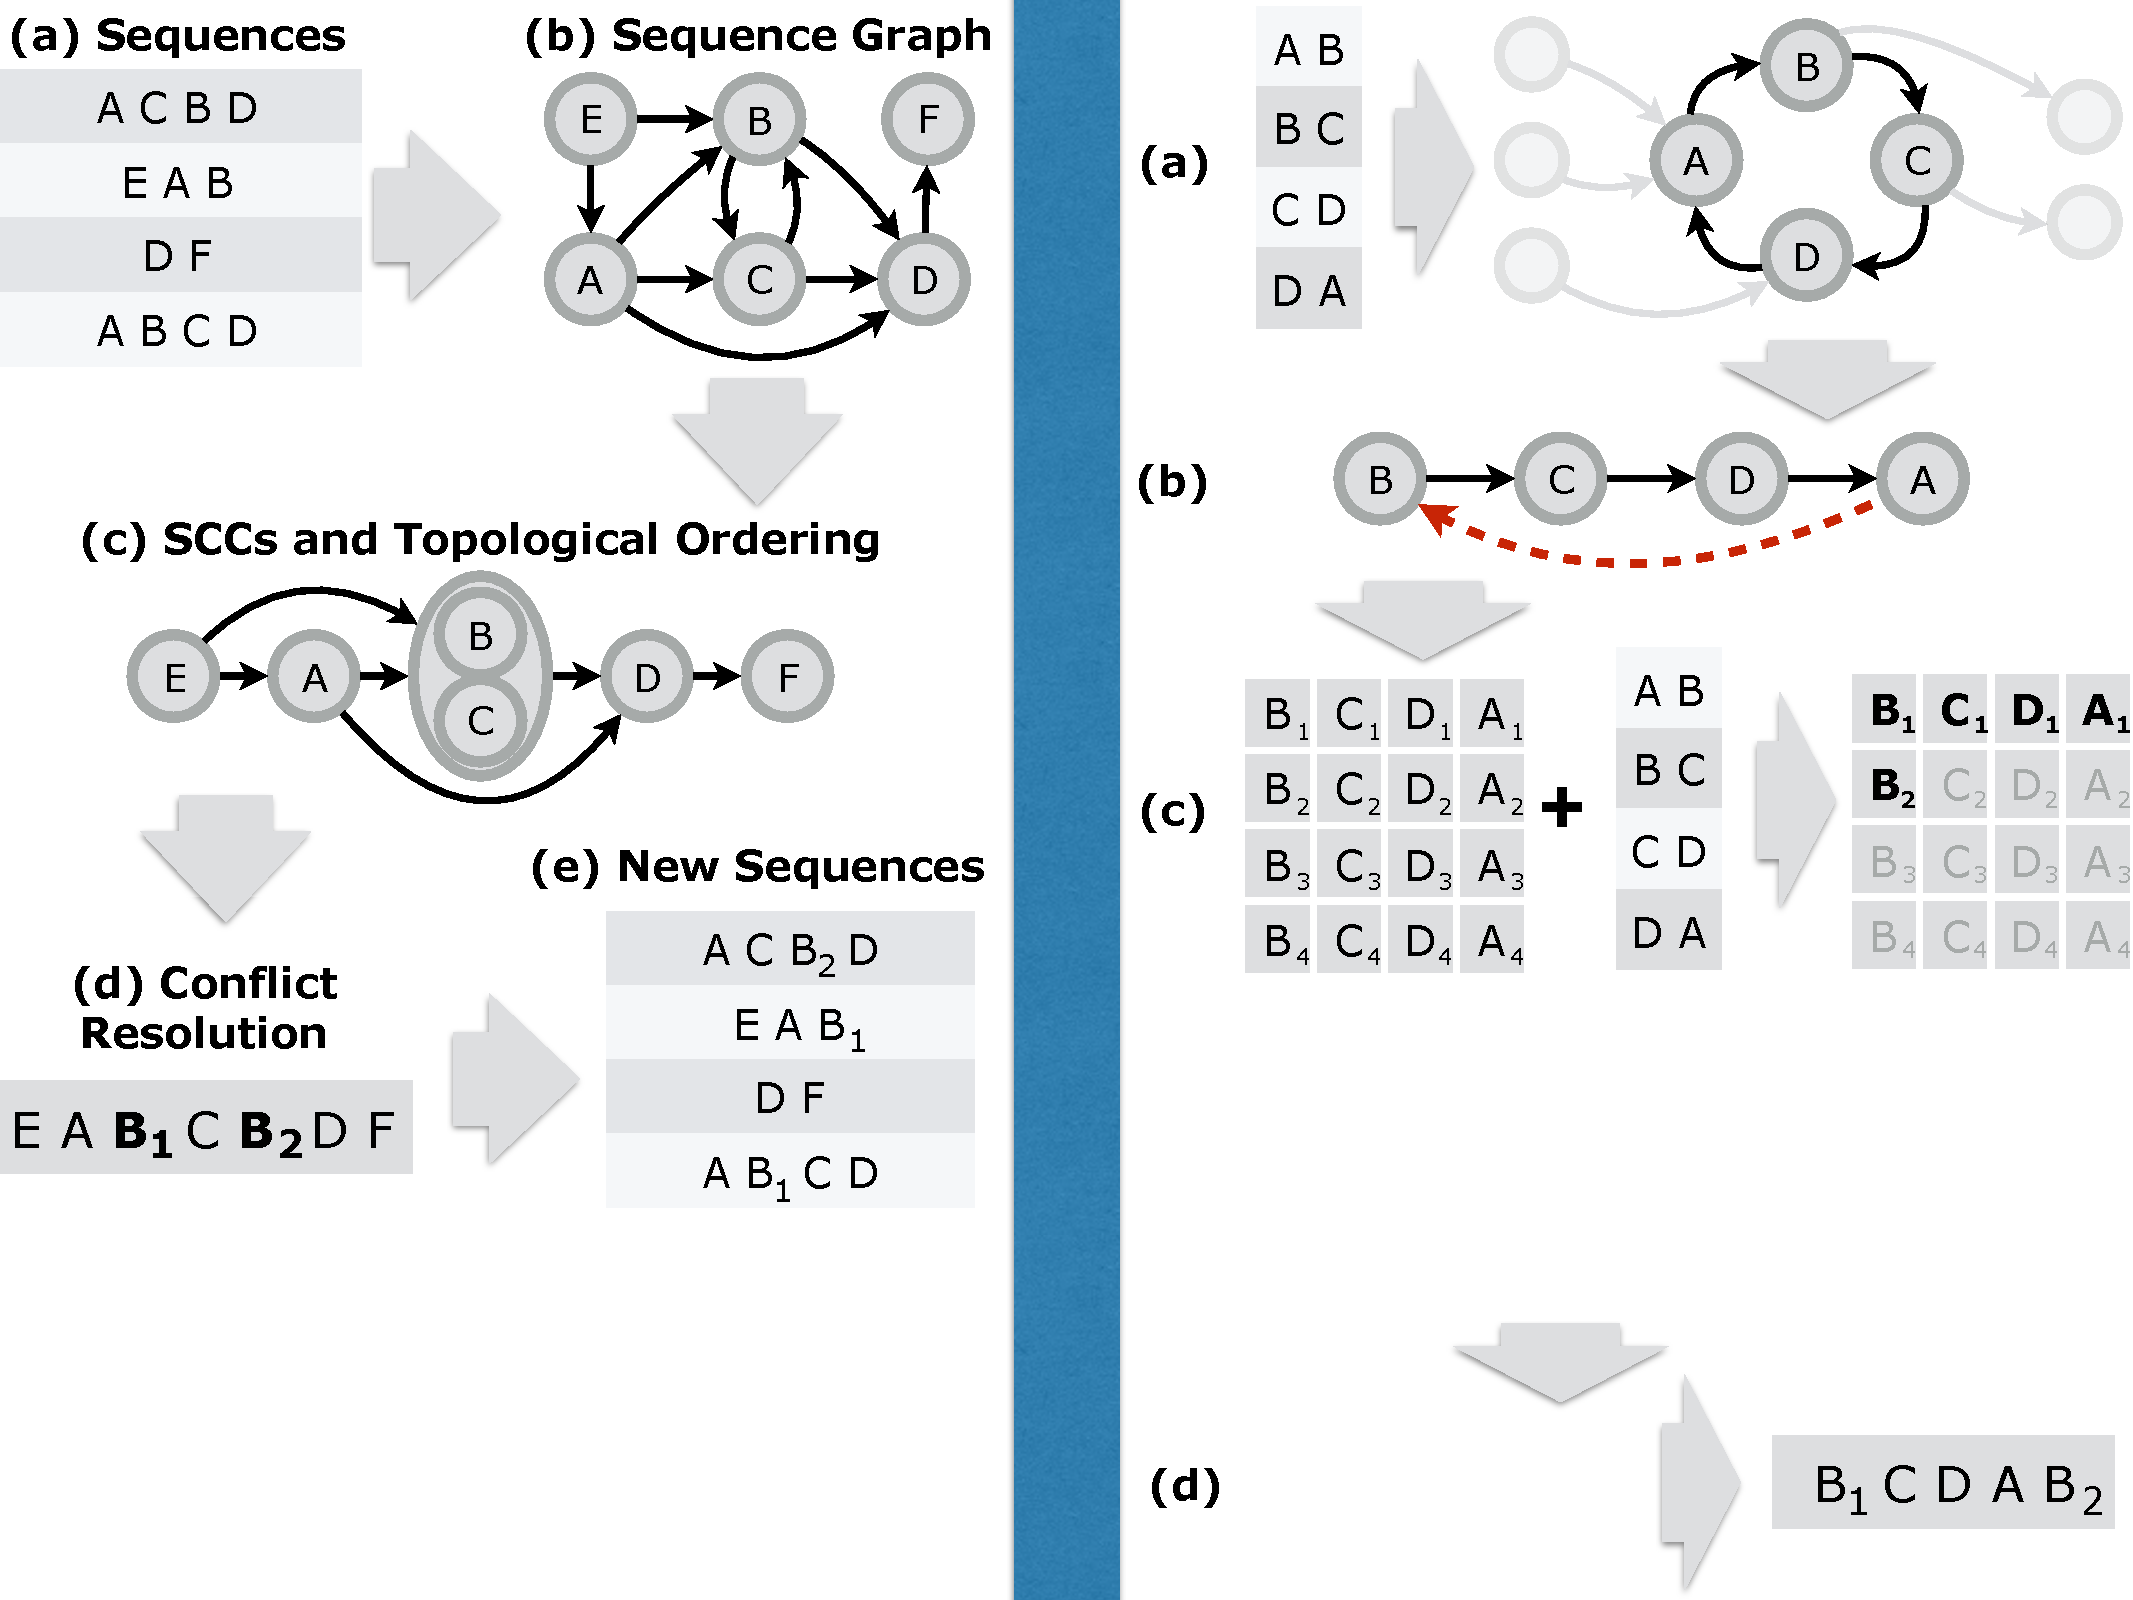
\includegraphics[trim={19.2cm 10cm 0 0}, clip, width=\linewidth]{figures/partial_ordering}
%\end{subfigure} 
%\end{minipage} 
%\caption{This details the order-inconsistency resolution step of the algorithm. (a) shows a SCC of four attributes. (b) shows an 'almost' ordering of the SCC nodes, which minimizes the number of backward edges. (c) shows a  construction of a worst-case quadratically-sized universe, which is then traversed by every sequence to determine which attributes to splits for the new ordering.}
%\label{fig:conflict_res}
%\end{figure}

\begin{figure*}[t!]
%\begin{minipage}{2\linewidth}
%\begin{subfigure}[c]{0.96\linewidth}
%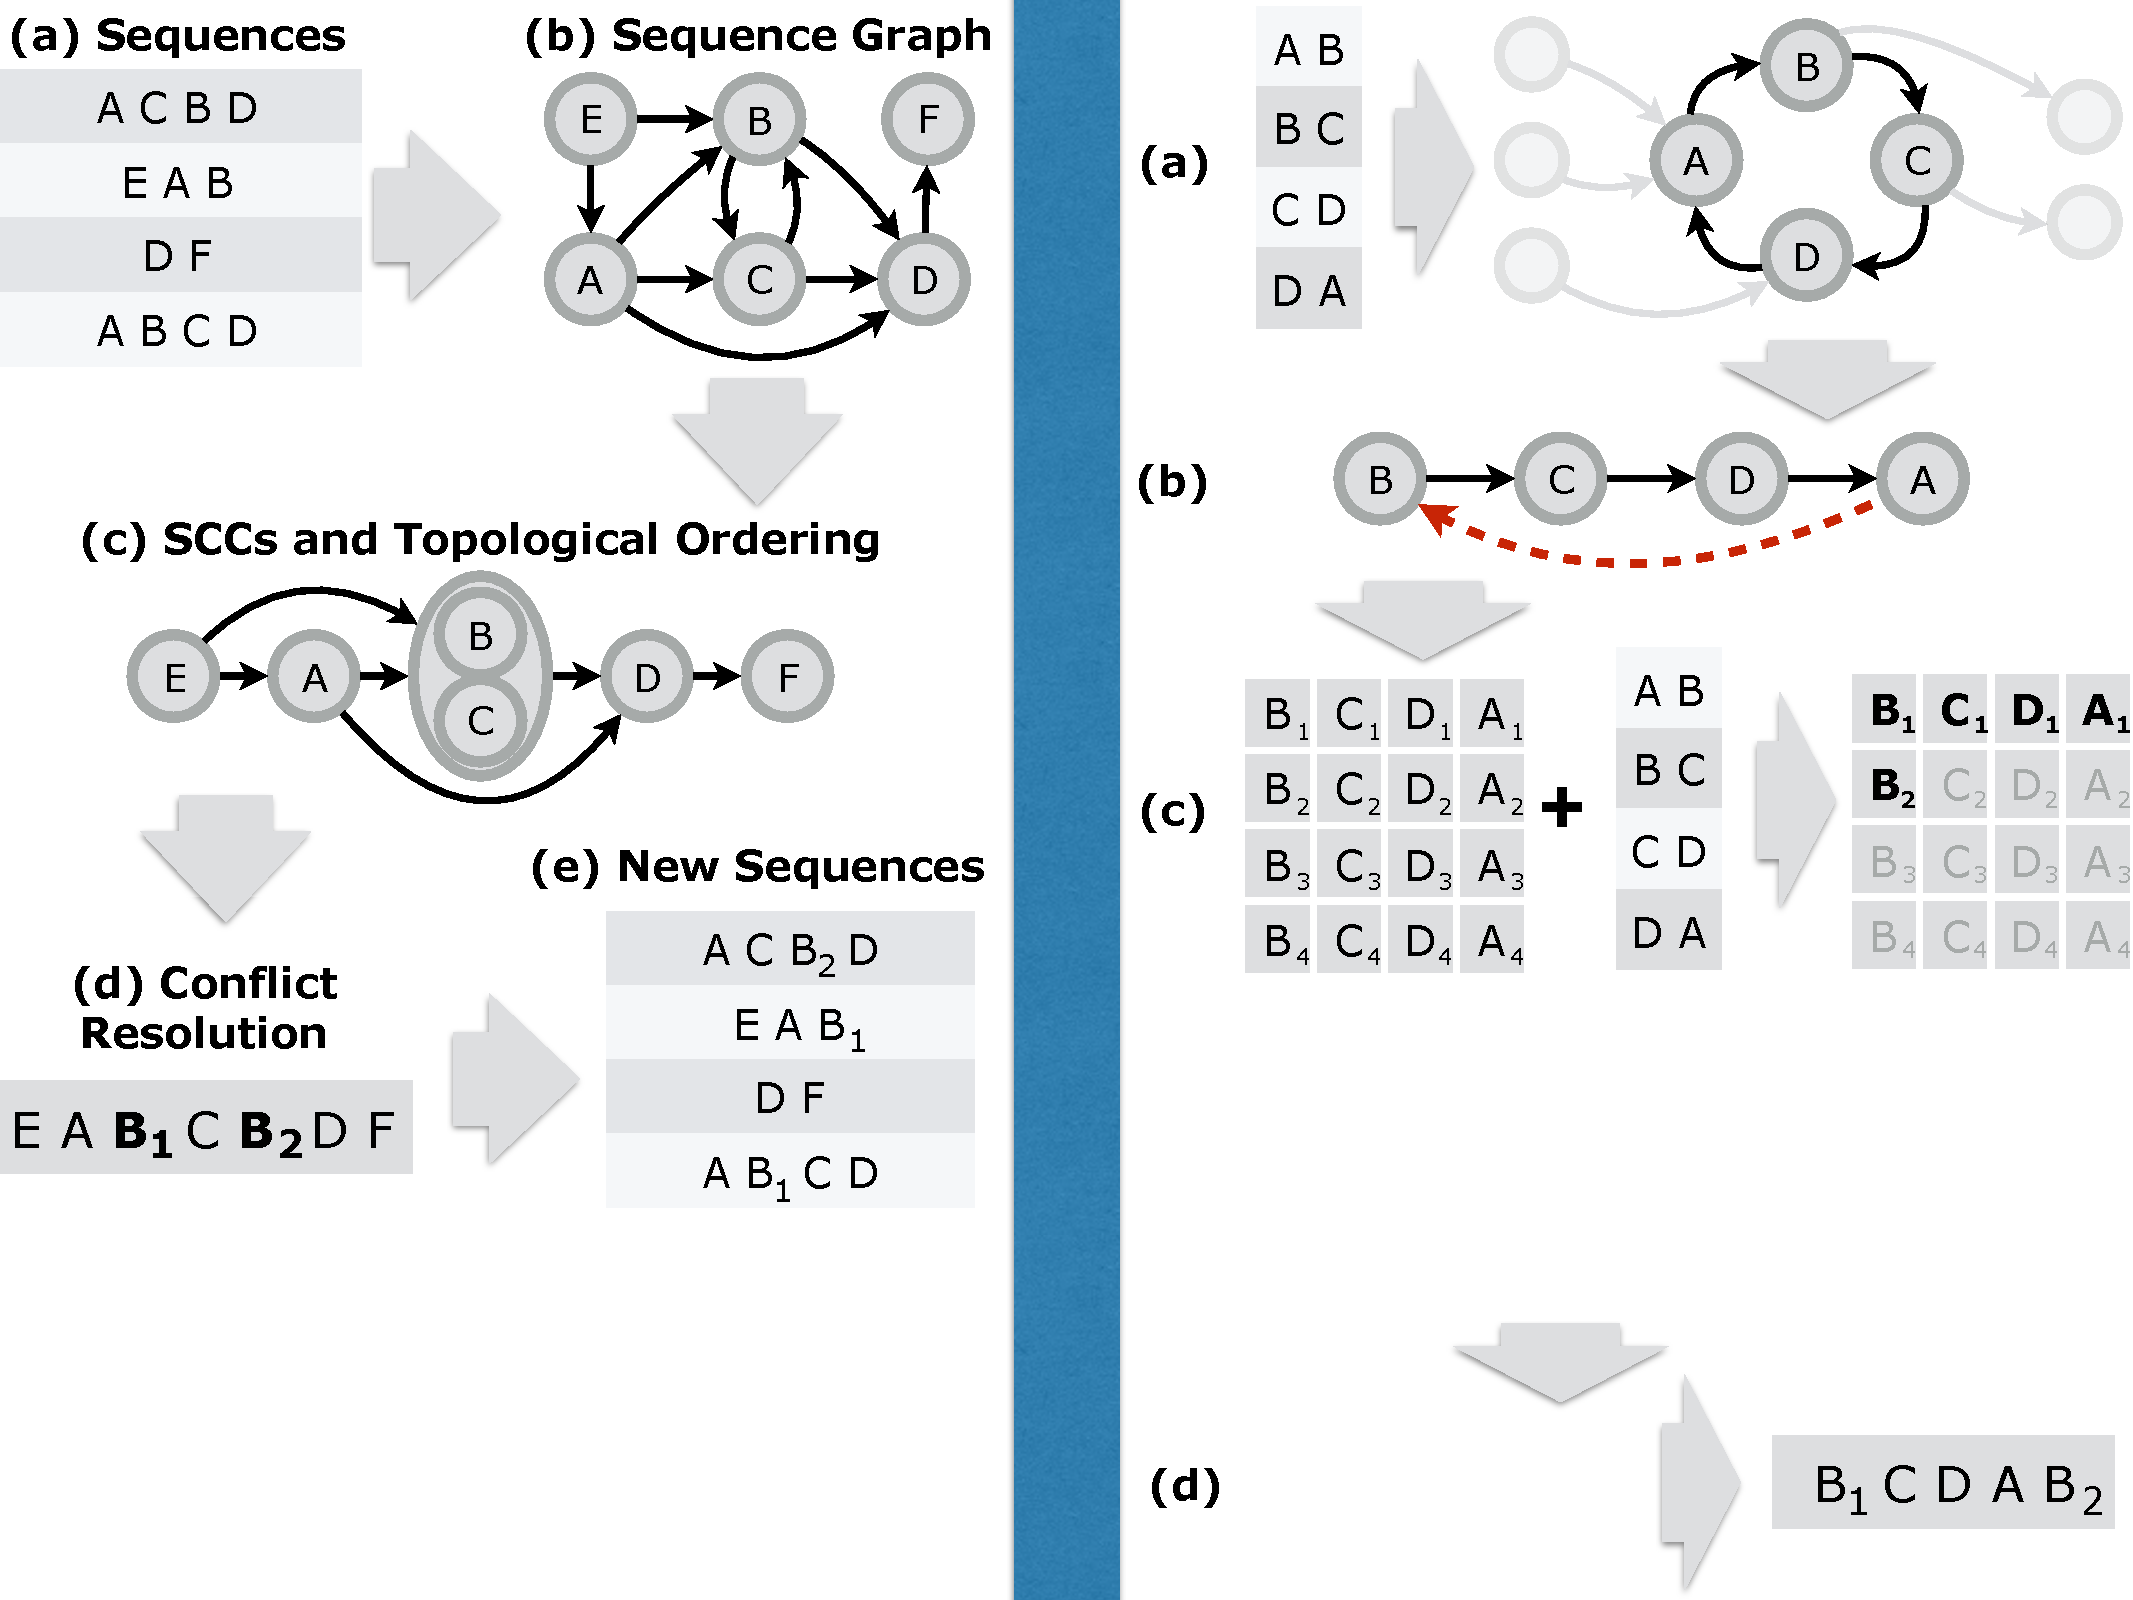
\includegraphics[trim={0 6cm 19.2cm 0}, clip, width=\linewidth]{figures/partial_ordering}
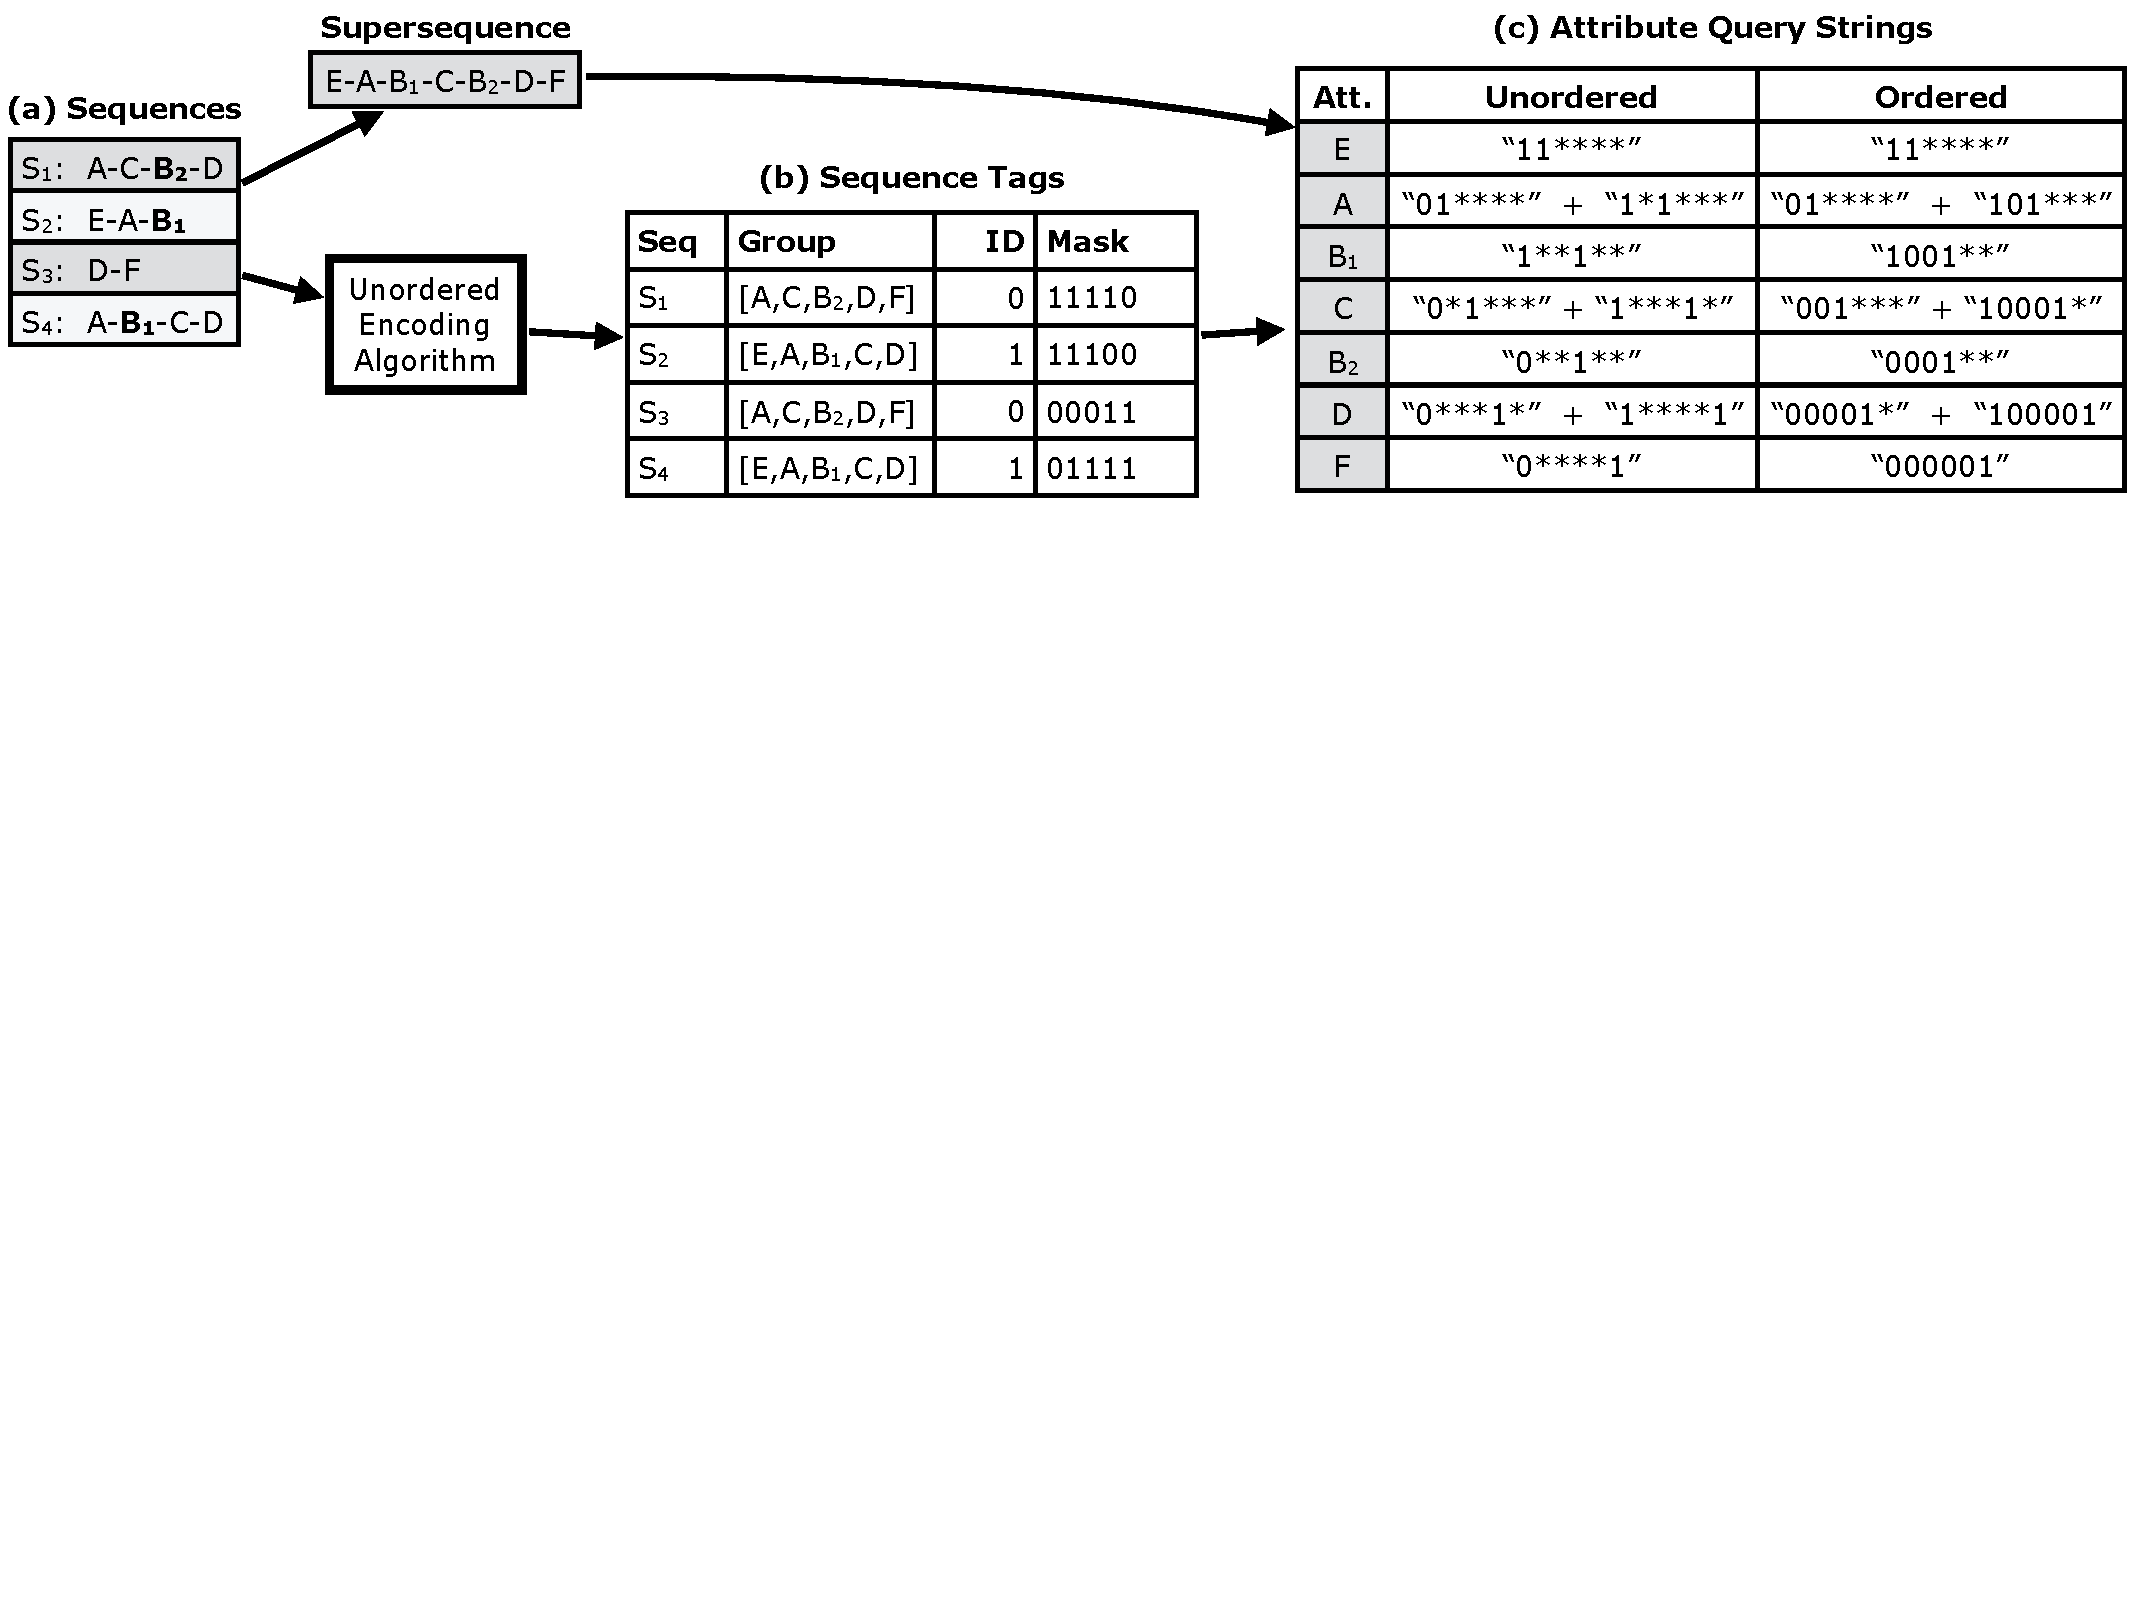
\includegraphics[trim={0 18cm 0 0}, clip, width=\textwidth]{figures/ordered_match_strings}
%\end{subfigure} 
%\end{minipage} 
\caption{Match strings for attribute sets versus sequences. (a) shows the set of input sequences which, when treated as unordered sets and run through Algorithm~\ref{alg:memory_min}, produce a set of tags in (b). The unordered column of (c) shows the query strings produced for checking each attribute in an unordered fashion. The ordered column is produced by taking the unordered strings and replacing wildcard characters with 0 for every attribute that appears before the current attribute in the ordering.}
\label{fig:ordered_rules}
\end{figure*}


\subsection{Constructing Rules That Respect Order}
\label{s:order-rules}

We previously showed how to construct tags and match strings for attribute \emph{sets}. Figure~\ref{fig:ordered_rules} shows the process for constructing rules for \emph{sequences} of attributes. The process assumes that the input sequences are drawn from a supersequence (as in Figure~\ref{fig:ordering}(g), shown again in Figure~\ref{fig:ordered_rules}(a)), so the input to this process is the output of the conflict-resolution algorithm described in \S~\ref{ss:breakcycle}.

The input sequences are treated as attribute \emph{sets} and run through our encoding scheme (Algorithm~\ref{alg:memory_min}), to produce a tag for each sequence (Figure~\ref{fig:ordered_rules}(b)) and a set of unordered match strings for each attribute (middle column of Figure~\ref{fig:ordered_rules}(c)) .  To produce \emph{ordered} rules from the unordered rules, we consider the concrete example of attribute $A$.  The unordered tests for $A$ include a rule for each group that contains $A$.  The first rule (``$01****$'') matches on group id $0$ and the first bit of the bitmask ($[A,C,B_2,D,F]$), and the second rule (``$1*1***$'') matches on group id $1$ and the second bit of the bitmask ($[E,A,B_1,C,D]$).

However, the the second rule is not appropriate when considering attributes in a \emph{sequence} because attribute $E$ appears ahead of $A$ in the sequence $E$-$A$-$B_1$-$C$-$D$.  If attribute $E$ holds for a packet (\ie, the bit for attribute $E$ is set to $1$), the packet should match a rule concerning attribute $E$ (\eg, ``$11****$'') rather than $A$.  So, policies that impose an ordering on the attributes must check that all \emph{earlier} attributes in the bitmask are set to $0$.  So, in the right column of Figure~\ref{fig:ordered_rules}(c), there is a match string for each group that contains $A$, with any bits \emph{before} $A$ in the bitmask set to $0$ rather than a wildcard.  That is, the second rule is ``$101***$'' for an ordered test on $A$, instead of the ``$1*1***$'' match for the unordered test.
